% ---------------------------------------------------------------
% CSCI 3010U -- Simulation and Modeling  |  Course Project
% 2D Billiards Physics Simulation Using Python
% Yash Patel  |  100785833  |  April 10, 2026
%
% HOW TO USE ON OVERLEAF:
%   1. Upload main.tex and preamble.tex
%   2. Upload: simulation_screenshot.png  and  experiment_summary.png
%   3. Click Compile
% ---------------------------------------------------------------

\documentclass[12pt, letterpaper]{article}

\usepackage[margin=1in]{geometry}
\usepackage[utf8]{inputenc}
\usepackage[english]{babel}
\usepackage[runin]{abstract}
\usepackage{titling}
\usepackage{fancyhdr}
\usepackage{graphicx}
\usepackage{parskip}
\usepackage{amsmath}
\usepackage{booktabs}
\usepackage{hyperref}
\usepackage{microtype}
\usepackage{enumitem}
\usepackage{setspace}

\input{preamble.tex}

% ---------------------------------------------------------------
\title{2D Billiards Physics Simulation Using Python}
\runningtitle{2D Billiards Simulation}
\author{Yash Patel}
\runningauthor{Y. Patel}
\affiliation{Ontario Tech University}
\department{Faculty of Science, Computer Science --- CSCI 3010U}
\memoid{Student Number: 100785833}
\theyear{2026}
\mydate{April 10, 2026}
% ---------------------------------------------------------------

\begin{document}
\maketitle
\thispagestyle{firstpage}

% ---------------------------------------------------------------
% Abstract
% ---------------------------------------------------------------
\begin{abstract}
\noindent
For my CSCI~3010U course project, I built a two-dimensional billiards
simulation using Python and the Pygame library.
The simulation places eight balls on a table and models their motion,
wall bouncing, and mutual collisions using real physics principles.
Ball positions are updated with the Euler method for numerical integration,
wall bouncing works by reversing the velocity perpendicular to the wall,
and ball--ball collisions are resolved using Newton's Law of Restitution
with an impulse-based approach.
A linear damping model simulates friction on the table surface.
Three controlled experiments were conducted to study how the restitution
coefficient and damping coefficient affect the total kinetic energy and
total momentum of the system over time.
All results matched the theoretical predictions from physics,
which confirms that the simulation is physically valid.
\end{abstract}

\noindent\textbf{Keywords:} Billiards, Euler method, numerical integration,
collision detection, Newton's Law of Restitution, damping,
kinetic energy, conservation of momentum

\medskip\hrule\medskip

% ---------------------------------------------------------------
\section{Introduction}
% ---------------------------------------------------------------

Computer simulations are one of the most powerful tools in science and
engineering.
They allow us to study physical systems that are too expensive, too
dangerous, or too complex to experiment on directly.
A good example of this is a billiards table: the physics of moving
balls, collisions, and energy loss are all well understood mathematically,
which makes billiards a great system to simulate and validate.

I chose billiards as my project topic because it connects directly to
the techniques we studied in CSCI~3010U, including numerical methods
for solving ordinary differential equations, rigid-body collision
detection and response, and energy analysis.
It is also a system where I can visually verify that the simulation
is behaving correctly --- if the balls move and bounce in a realistic
way, that is already strong evidence the physics is right.

The goal of my project was to build a simulation that handles four
main tasks:

\begin{enumerate}[noitemsep]
  \item Update each ball's position using a numerical method
        (the Euler method) at every time step.
  \item Detect and respond to ball--wall collisions using
        velocity reversal.
  \item Detect and resolve ball--ball collisions using
        conservation of momentum and Newton's Law of Restitution.
  \item Apply a friction (damping) model to gradually reduce
        the speed of all balls over time.
\end{enumerate}

Beyond building the simulation, I also ran three experiments to
measure how the system behaves under different physical parameters.
The results were compared against what physics theory predicts to
validate that the simulation is correct.

This type of simulation is relevant to many real-world applications.
Game engines use the same physics principles for collision handling.
Engineering software uses similar methods to simulate mechanical
systems.
And in education, interactive simulations like this one help students
understand abstract physics concepts in a concrete, visual way.

% ---------------------------------------------------------------
\section{Background and Physics Principles}
% ---------------------------------------------------------------

This section explains the physics and mathematics used in the
simulation.
All of these topics were covered in the CSCI~3010U course lectures,
and I applied them directly in my project.

\subsection*{Numerical Integration --- the Euler Method}

A ball's motion is governed by ordinary differential equations (ODEs).
To simulate motion on a computer, these continuous equations must be
approximated using a discrete time step $\Delta t$.
The simplest approach is the \textbf{Euler method}:
\begin{align}
  x(t+\Delta t) &= x(t) + v_x(t)\cdot\Delta t \label{eq:euler_x}\\
  y(t+\Delta t) &= y(t) + v_y(t)\cdot\Delta t \label{eq:euler_y}
\end{align}
The Euler method is a first-order method, which means it uses only
the current velocity to predict the next position.
I chose it for this project because it is simple to implement and
computationally efficient, making it well-suited to a real-time simulation
running at 120 frames per second.
The main trade-off is that the Euler method introduces a small numerical
error at each step --- the position estimate is slightly off compared to
the true analytical solution.
However, because the time step I use is small ($\Delta t = 1/120\,\text{s}$),
this error is negligible and does not affect the visual realism of the
simulation.
If higher accuracy were needed --- for example in scientific computation ---
a higher-order method such as Runge--Kutta (RK4) would be preferred.

\subsection*{Damping --- Simulating Friction}

In real billiards, friction between the ball and the table cloth
causes the balls to slow down over time.
I model this with a linear damping equation applied to the velocity
at each time step:
\begin{equation}
  v(t+\Delta t) = v(t)\cdot(1 - \lambda\,\Delta t)
\end{equation}
where $\lambda \geq 0$ is the damping coefficient.
When $\lambda = 0$ there is no friction and balls roll forever.
A larger $\lambda$ causes faster slowing.
This model is equivalent to an exponential decay of speed over time,
which is consistent with the behaviour of linear drag forces.

\subsection*{Ball--Wall Collisions}

When a ball's edge reaches the boundary of the table,
it bounces back.
I implement this by reversing the velocity component that is
perpendicular to the wall it just hit:
\begin{itemize}[noitemsep]
  \item Left or right wall: $v_x \leftarrow -v_x$
  \item Top or bottom wall: $v_y \leftarrow -v_y$
\end{itemize}
After reversing the velocity, the ball is repositioned so it no longer
overlaps with the wall.
This positional correction prevents a bug known as
\textit{tunnelling}, where a fast-moving ball could pass through
the wall entirely in a single time step.
All wall collisions in the simulation are perfectly elastic --- the ball
loses no kinetic energy when bouncing off a wall.

\subsection*{Ball--Ball Collisions}

Two balls are colliding when the distance between their centres
is less than the sum of their radii:
\begin{equation}
  d = \sqrt{(x_2-x_1)^2 + (y_2-y_1)^2} < r_1 + r_2
\end{equation}

To resolve the collision, I compute a unit normal vector $\hat{n}$
pointing from ball~1 toward ball~2, and the relative velocity along
that normal:
\begin{equation}
  dv_n = (\mathbf{v}_1 - \mathbf{v}_2)\cdot\hat{n}
\end{equation}
If $dv_n \leq 0$, the balls are already moving apart and no action
is needed.
Otherwise, the impulse magnitude is given by Newton's Law of
Restitution:
\begin{equation}
  J = \frac{-(1+e)\cdot dv_n}{\dfrac{1}{m_1}+\dfrac{1}{m_2}}
  \label{eq:impulse}
\end{equation}
where $e$ is the coefficient of restitution ($0 \le e \le 1$).
The impulse $J$ acts along the collision normal $\hat{n}$ and
redistributes velocity between the two balls ---
a faster ball slows down and a slower ball speeds up,
exactly as in a real collision.
The velocities are updated as:
\begin{align}
  \mathbf{v}_1 &\mathrel{+}= (J/m_1)\,\hat{n} \\
  \mathbf{v}_2 &\mathrel{-}= (J/m_2)\,\hat{n}
\end{align}
When $e = 1$ the collision is perfectly elastic: total kinetic energy
is conserved.
When $e < 1$ some kinetic energy is lost (converted to heat or sound),
which is the case in real billiards.

The total kinetic energy of the system at any point is:
\begin{equation}
  KE_{\text{total}} = \sum_{i=1}^{N} \tfrac{1}{2}\,m_i\,v_i^2
  \label{eq:ke}
\end{equation}

% ---------------------------------------------------------------
\section{Implementation}
% ---------------------------------------------------------------

I structured my project across three Python files, keeping each
file focused on a specific responsibility.

\textbf{\texttt{ball.py} --- Ball class.}
This file defines the \texttt{Ball} class.
Each ball stores its position $(x, y)$, velocity $(v_x, v_y)$,
radius, mass, and colour.
The \texttt{update(dt, damping)} method applies the damping equation
and then advances the position using the Euler method
(Equations~\ref{eq:euler_x} and \ref{eq:euler_y}).
The \texttt{wall\_collision()} method checks all four walls and,
where needed, reverses the velocity and corrects the position.
The \texttt{kinetic\_energy()} method returns $\frac{1}{2}mv^2$
for that ball.

\textbf{\texttt{physics.py} --- Collision engine.}
This file contains the \texttt{resolve\_ball\_collision(b1, b2, e)}
function.
It computes the distance between two balls,
builds the unit normal vector,
checks whether the balls are approaching,
computes the impulse $J$ using Equation~\ref{eq:impulse},
applies the velocity changes to both balls,
and then separates the balls to remove any remaining overlap.
It also contains helper functions to compute the total kinetic energy
and total momentum vector of all balls.

\textbf{\texttt{main.py} --- Interactive simulation.}
This file initialises the Pygame window (1130$\times$710 pixels)
and runs the main loop at 120 frames per second.
Each frame it: updates all ball positions, checks wall collisions,
checks all ball-pair collisions (brute-force $O(n^2)$ check),
and redraws everything.
The right-hand HUD panel shows the total kinetic energy,
elapsed time, collision count, current damping and restitution values,
and a live kinetic-energy graph.
Table parameters can be changed in real time using keyboard shortcuts:
\texttt{$\uparrow$/$\downarrow$} adjust damping,
\texttt{$\leftarrow$/$\rightarrow$} adjust restitution,
\texttt{SPACE} pauses, and \texttt{R} resets.

\textbf{\texttt{analysis.py} --- Experiment runner.}
This script runs the simulation without any display window
(``headless'' mode) and records kinetic energy and momentum data
over 12 seconds of simulated time.
It uses \texttt{matplotlib} to save the results as PNG graph files.

Figure~\ref{fig:screenshot} shows the simulation running.

\begin{figure}[ht]
  \centering
  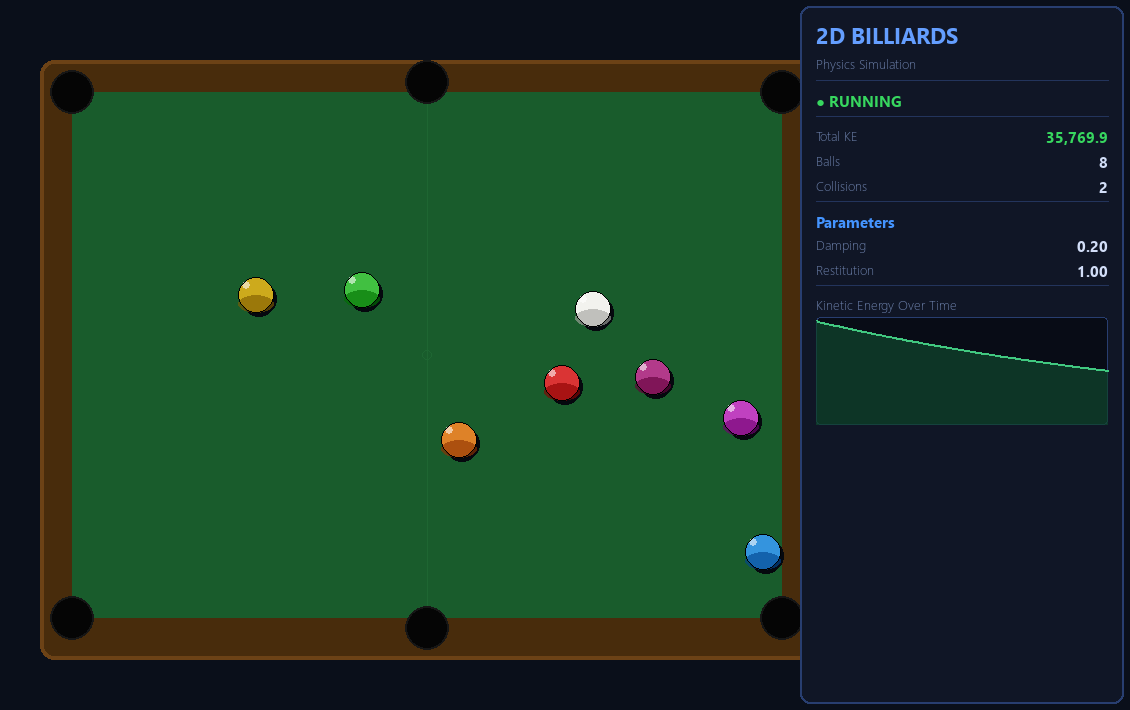
\includegraphics[width=0.90\linewidth]{simulation_screenshot.png}
  \caption{The interactive 2D billiards simulation.
    Eight colour-coded balls move on a green felt table.
    The right panel shows the live kinetic energy graph,
    collision counter, elapsed time, and the current values of
    the damping and restitution parameters.}
  \label{fig:screenshot}
\end{figure}

% ---------------------------------------------------------------
\section{Experiments and Results}
% ---------------------------------------------------------------

I ran three experiments using \texttt{analysis.py}
to test whether the simulation produces physically correct results.
All experiments begin with the same set of eight balls at the same
starting positions and velocities (controlled by a fixed random seed)
so that the results are directly comparable.
Each experiment runs for 12 seconds of simulated time.
Figure~\ref{fig:results} shows the output of all three experiments.

\subsection*{Experiment 1 --- Effect of Restitution on Kinetic Energy}

\textbf{Setup:} Three restitution values were tested:
$e = 1.0$ (perfectly elastic), $e = 0.7$ (moderately inelastic),
and $e = 0.4$ (highly inelastic).
Damping was set to zero ($\lambda = 0$) so that friction would not
interfere with the results.

\textbf{Results:}
When $e = 1.0$, the total kinetic energy stays perfectly constant
throughout the entire 12 seconds.
This confirms that elastic collisions conserve kinetic energy as expected.
When $e = 0.7$, the energy decreases in visible steps.
Each step on the graph corresponds to one ball--ball collision,
and each collision removes some energy from the system.
When $e = 0.4$, the steps are much larger --- more energy is lost
per collision --- and the total energy drops more quickly.

\textbf{Conclusion:}
The simulation correctly implements Newton's Law of Restitution.
Lower restitution causes more kinetic energy to be dissipated
per collision, which matches the physics formula in
Equation~\ref{eq:impulse}.

\subsection*{Experiment 2 --- Effect of Damping on Kinetic Energy}

\textbf{Setup:} Three damping values were tested:
$\lambda = 0.0$ (no friction), $\lambda = 0.2$ (light friction),
and $\lambda = 0.6$ (heavy friction).
Restitution was set to $e = 1.0$ (elastic) so that only damping
affected the energy.

\textbf{Results:}
With no damping the kinetic energy remains constant -- balls roll
forever.
With $\lambda = 0.2$, energy decays smoothly over time,
following an exponential curve.
With $\lambda = 0.6$ the decay is much steeper and the balls
effectively stop within about four seconds of simulation time.

\textbf{Conclusion:}
The exponential decay of kinetic energy matches the analytical
solution of the damping ODE.
A higher damping coefficient removes energy faster, which is exactly
what the linear friction model predicts.

\subsection*{Experiment 3 --- Total Momentum Over Time}

\textbf{Setup:}
The magnitude of total system momentum was tracked over 12 seconds
using elastic collisions and no damping.

\textbf{Results:}
The momentum plot shows sudden discrete changes.
These jumps happen every time a ball hits the table wall.
The wall applies an external force on the ball, which changes the
system's momentum.
Between wall hits, whenever two balls collide with each other,
the total momentum does \emph{not} change --- the impulse that one
ball receives is equal and opposite to what the other ball receives,
so the total cancels out.

\textbf{Conclusion:}
Ball--ball collisions conserve total linear momentum, which is
consistent with Newton's Third Law.
Momentum only changes due to external forces (the walls),
as expected.

\begin{figure}[ht]
  \centering
  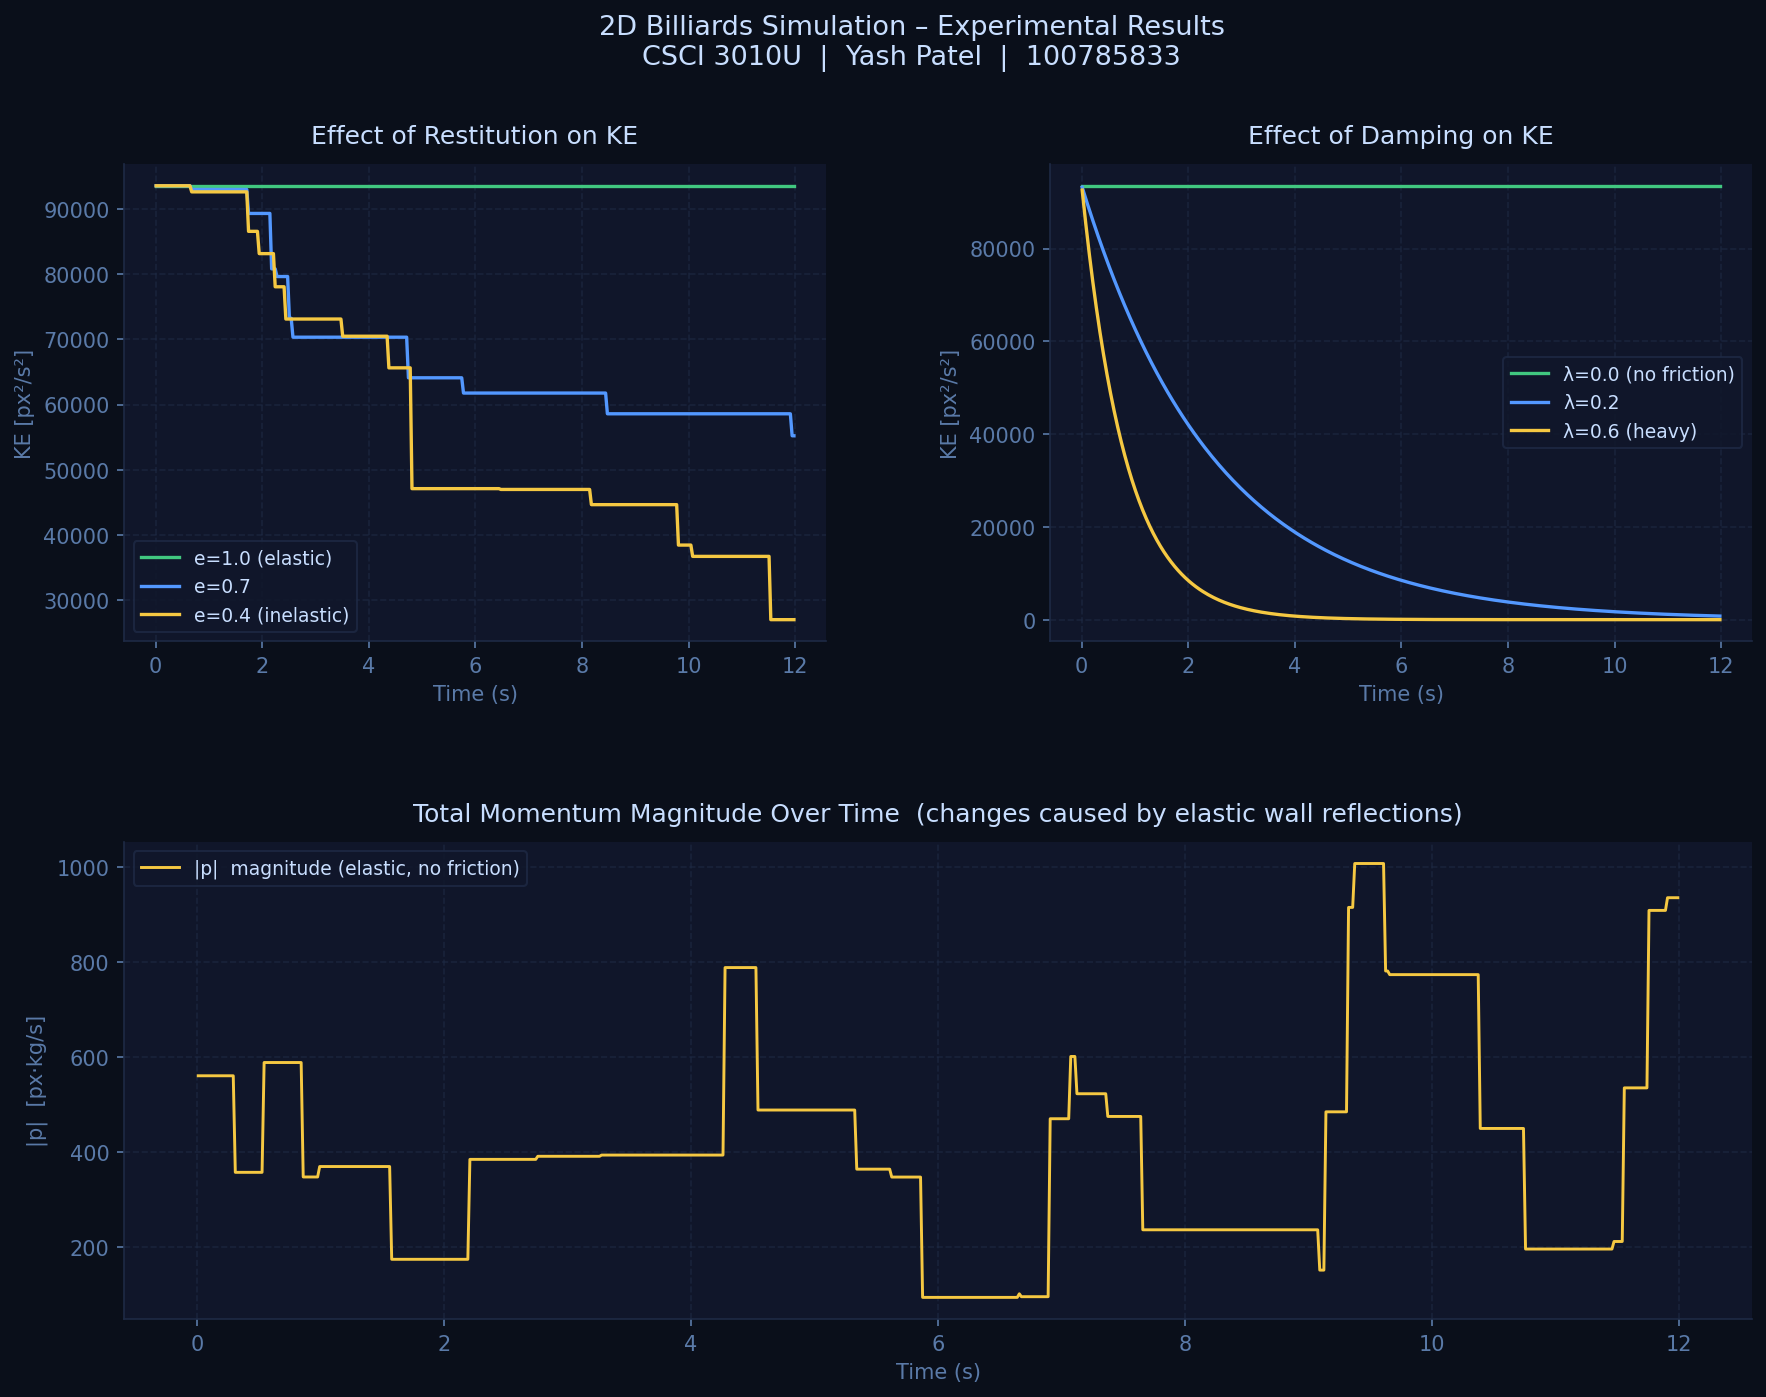
\includegraphics[width=0.97\linewidth]{experiment_summary.png}
  \caption{Summary of all three experiments.
    \textit{Top-left:} total kinetic energy over time for three
    restitution values (no damping).
    \textit{Top-right:} total kinetic energy over time for three
    damping values (elastic collisions).
    \textit{Bottom:} total momentum magnitude over time
    (elastic, no friction). Jumps correspond to wall collisions.}
  \label{fig:results}
\end{figure}

% ---------------------------------------------------------------
\section{Discussion}
% ---------------------------------------------------------------

Overall, all three experiments produced results that match what
physics theory predicts, which tells me the simulation is working
correctly.
There are, however, a few things I want to reflect on.

\textbf{Numerical accuracy of the Euler method.}
The Euler method introduces a small amount of numerical error at
each time step because it uses a linear approximation of a
continuous curve.
In a long simulation with large time steps this could cause balls
to gain or lose energy slightly even in a perfectly elastic system.
In my simulation I keep $\Delta t = 1/120\,\text{s}$ which is small
enough that this error is not visible.
I verified this by checking that the kinetic energy stays flat
when $e = 1$ and $\lambda = 0$ (Experiment~1, top-left graph).
If I were to extend this project, I would switch to the RK4 method
for more precise integration.

\textbf{Brute-force collision detection.}
My simulation checks every pair of balls for collision at every
frame, which is an $O(n^2)$ approach.
For 8 balls this is 28 checks per frame and works fine.
For hundreds of balls it would become slow.
A more scalable approach would use spatial partitioning
(such as a grid or a quadtree) to only check nearby pairs.

\textbf{Wall collision energy.}
In the simulation, walls are treated as immovable fixed boundaries.
This means the wall does not absorb any energy --- all energy loss
at walls comes purely from reversing velocity.
In a real billiards game the cushions (rails) do absorb some energy,
which could be modelled by giving walls their own restitution value.

% ---------------------------------------------------------------
\section{Conclusion}
% ---------------------------------------------------------------

This project gave me hands-on experience applying the simulation
techniques taught in CSCI~3010U to a real physical system.
I implemented the Euler method for numerical integration of ball motion,
elastic velocity reversal for wall bouncing, impulse-based ball--ball
collision resolution using Newton's Law of Restitution,
and a linear damping model for friction.

All three experiments confirmed that the simulation is physically valid:
\begin{itemize}[noitemsep]
  \item Elastic collisions ($e=1$) conserved kinetic energy exactly.
  \item Inelastic collisions ($e<1$) dissipated energy in proportion
        to the restitution value.
  \item Damping caused smooth exponential decay of kinetic energy.
  \item Momentum was conserved between ball--ball collisions and
        only changed at wall reflections.
\end{itemize}

If I were to continue this project, I would add proper pocket detection
so balls can be ``potted'', implement RK4 integration for better
numerical accuracy, and use spatial partitioning to support more balls
efficiently.
Overall, building this simulation helped me connect the physics equations
from lectures to actual working code, which was a valuable learning
experience.

% ---------------------------------------------------------------
\begin{thebibliography}{9}

\bibitem{gould2007}
H.~Gould, J.~Tobochnik, and W.~Christian,
\textit{An Introduction to Computer Simulation Methods:
Applications to Physical Systems}, 3rd~ed.
Addison-Wesley, 2007.

\bibitem{course-notes}
Course Notes,
\textit{CSCI 3010U -- Simulation and Modeling},
Ontario Tech University, 2026.
Available at: \url{http://csundergrad.science.uoit.ca/courses/sim-and-modeling-notes/}

\bibitem{pygame}
Pygame Community,
\textit{Pygame Documentation}.
\url{https://www.pygame.org/docs/}, Accessed April 2026.

\bibitem{ericson2004}
C.~Ericson,
\textit{Real-Time Collision Detection}.
Morgan Kaufmann, 2004.

\end{thebibliography}

\end{document}